\documentclass[12pt,a4paper]{article}
\usepackage[utf8]{inputenc}

\usepackage{geometry}
\usepackage{setspace}
\usepackage{amsmath}
\usepackage[margin=1cm]{caption}
\usepackage{titling}
\usepackage{parskip}
\usepackage{booktabs}
\usepackage{fancyhdr}
\usepackage{lipsum}

\geometry{margin=.95in}
\onehalfspacing

\title{A decentralized insurance and reinsurance marketplace\\\vspace{5mm}\small\textit{V0.3}\vspace{20mm}}
\author{\textbf{Authors}\\Stephan Karpischek\\Christoph Mussenbrock\\Jake Brukhman\\Ron Bernstein\\\\\textbf{Reviewed by:}\\Chris Padovano\\Aleksandr Bulkin\\Alexander Felix\\\\}
\usepackage{natbib}
\usepackage{graphicx}
\usepackage{titling}
\usepackage{float}
\usepackage{graphicx}
\graphicspath{ {images/} }
\usepackage{tocloft}
\usepackage{cals}
% Turn on the style
\pagestyle{fancy}
% Clear the header and footer
\fancyhead{}
\fancyfoot{}
% Set the right side of the footer to be the page number
\fancyfoot[R]{Page \thepage}
% add horizontal line
\renewcommand{\footrulewidth}{0.4pt}

\begin{document}
\setcounter{page}{43}

\appendix
\renewcommand{\thesection}{\arabic{section}}
\setcounter{section}{7}
\section{Appendix}
\setcounter{subsection}{1}
\newpage
\subsection{Credit Risk Model}

\subsubsection{Abstract}

This is a technical addendum to the Etherisc\footnote{http://etherisc.com} decentralized insurance whitepaper, presented at the EtherCamp Virtual Accelerator (http://hack.ether.camp). In this work, we develop a simple probability model for a parametric insurance pool with variable claim payouts and variable probabilities of insurable events. We present one methodology for calculating premiums. We also suggest avenues for employing this model in a real-time context of a portfolio that continuously underwrites claims. Finally, we present a Python simulation which puts our modeling methodology into practice against actual data for insurable flight delays.

\subsubsection{Overview}

In this section, we describe the desirable properties of a basic credit risk model for decentralized insurance with a minimum viable set of features that can enable the proof of concept Etherisc application. In general, insurance works by selling policies which cost the purchaser a premium in exchange to an entitlement to a payout in the case of some \textit{insurable event}. The occurrence of the event and subsequent automated payout is referred to as a \textit{claim}. The Etherisc demo application focuses on the case of flight delays, but in our model we do not make any assumption about the specific nature of the event with an eye to expanding our insurance offering to different markets.

An insurance risk pool underwrites policies by taking on some maximum liability in the form of credit for potential claims, and collateralizing the portfolio with a smaller amount of capital to cover the capital outflow due to claims with a reasonable confidence level. If the portfolio experiences a capital outflow of claims which exceeds the collateralization of the risk pool, the risk pool becomes insolvent. This problem of excess risk management is addressed by the Etherisc whitepaper and its decentralized reinsurance market based on cryptographic tokens.

We target the following mathematical properties in our model of an insurance risk pool:

\begin{enumerate}
\item The portfolio should be able to reasonably model insurable events as independent (and uncorrelated) random variables.
\item The model should be able to provide distinct probabilities of each individual event as parameters.
\item The portfolio should be able to underwrite policies for an arbitrary payout amount.
\item The model should be able to parametrize the probability of solvency of the portfolio at an arbitrarily high confidence level.  
\end{enumerate}

In modeling insurance, correlation analysis of events plays a key role in achieving highly realistic models but significantly increases model complexity. For the purposes of our proof of concept product, we assume independence of insurable events and offload the risk due to error to our reinsurance market (covered in the Etherisc whitepaper). We recognize the importance of correlation analysis and future efforts will focus on developing more granular modeling methodologies. Note that this model's ability to underwrite payouts of arbitrary size is crucial because it enables the risk pool underwrite multiple policies pertaining to the same event without requiring a model based on correlated random variables.

In general, we also desire that our model outputs should cover the gamut of relevant financials that might be useful in constructing a smart contract\footnote{Decentralized insurance rests on the idea of a decentralized implementation on a smart contract platform such as Ethereum. See: http://ethereum.org.} which manages the insurance pool: (i) the total liability of the credit portfolio; (ii) the required collateralization of the risk portfolio; (iii) at least one plausible method for calculating premiums commensurate with event probabilities and payouts; and (iv) an expectation and spread for the revenue of the portfolio (ideally, non-negative).

Finally, our model should be straightforward to calculate (or estimate). In the following section, we develop the mathematics for a model which conforms to the properties above.

\subsubsection{Probability model}

Let us assume that our risk pool portfolio contains $n$ policies which are insuring against $n$ insurable events, modeled as independent but not necessarily identically distributed random variables $X_i$ $(i=1,\ldots,n)$. Suppose that $P^*_i$ $(i=1,\ldots,n)$ is a fixed set of desired payouts where $P^*_i$ corresponds to the policy $i$. Furthermore, suppose that $X_i\in\{0,1\}$ are Bernoulli random variables with event probability $p_i$ $(i=1,\ldots,n)$. That is, $P(X_i = 1) = 1 - P(X_i = 0) = p_i$ for $i = 1,\ldots,n$. 

The \textit{total liability} $L$ of the portfolio is the sum of all payouts the portfolio is underwriting, and we define 
% %
% %
   $$L(n) := \sum_{i=1}^n P^*_i.$$
% %
% %
% We are interested to find the \textit{required collateral} $C(n)$, that is, the amount of capital the portfolio will hold to handle capital outflows due to claims. Typically, $C(n)/L(n)<1$, reflecting the fact that the portfolio is taking on credit risk. Our goal is to keep enough collateral in the portfolio to be able to pay a reasonably expected number of policy claims. We define the total capital outflow due to claims as
% %
% %
%   $$X:=\sum_{i=1}^n X_i P_i^*.$$ 
% %
% %
$X$ is a random variable that has a non-trivial distribution which is the weighted sum of Bernoulli variables with non-uniform probabilities. Let us define $\pi$ to be the desired confidence level (probability) of portfolio solvency, and we note that typically $\pi$ will be high ($\pi\approx 1$). Let $F_X$ be the cumulative distribution function of $X$. Our model is then defined by setting the required collateral $C$ to the $\pi$-percentile probable capital outflow due to claims:
% %
% %
\begin{equation}
    \label{model}
    C(n) = F_X^{-1}(\pi).
\end{equation}
% %
% %
Let us now to turn to calculating the set of premiums $P_i$ $(i=1,\ldots,n)$. For one, we must have that $\sum_{i=1}^n P_i = C(n) = F_X^{-1}(\pi)$, but we are free to choose how to distribute the claim costs among policies. While there are multiple ways to distribute the collateralization cost, we choose a method that has naturally desirable properties: (i) the premium $P_i$ should be proportional to the payout $P_i^*$ (intuitively, the higher the payout of a policy, the more the upfront premium cost); (ii) the premium $P_i$ should be proportional to the insurable event probability $p_i$ (intuitively, the lower the probability of the event, the cheaper the premium). To achieve this relationship, set
% %
% %
     $$P_i := \frac{p_iP_i^*}{\sum_j p_jP_j^*} F_X^{-1}(\pi)$$
% %
% %
and it is clear that (\ref{model}) holds. Moreover, it is easy to check that $P_i \to 0$ as $\pi \to 0$ and $P_i\to\infty$ as $P_i^*\to\infty$ as required. If we find that at a small $n$ our premiums are too expensive, we have the option of reducing premiums with some initial subsidy capital seeded into the risk pool; however, we will not pursue the mathematical details of this extension as we believe premiums will already be sufficiently small.

A straightforward calculation shows that the expected value and standard deviation of $X$ are given by
% %
% %
  $$E(X) = \sum_{i=1}^np_iP_i^*\ ;\ \ \sigma_X = \sqrt{\sum_{i=1}^np_i(1-p_i)(P_i^*)^2}.$$
% %
% %
\begin{figure}[H]
    \begin{center}
        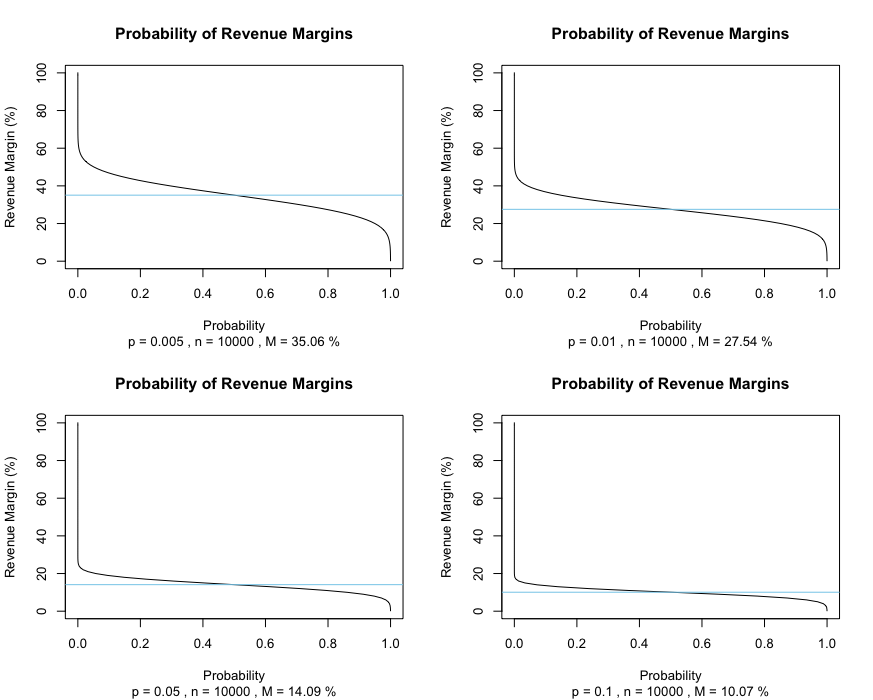
\includegraphics[scale=.5]{margins}
    \end{center}
    \caption{\footnotesize Probability distributions of revenue margins given different values of average event probability $p$. $M$ is the \textit{revenue margin}, the difference between capital outflows due to claims and the collateral $C$, divided by $C$.}\label{fig1}
\end{figure}
% %
% %
We now demonstrate that, given collateralization, our model produces a non-zero expectation of revenue with $\pi$-confidence. To show this, let us define the revenue $R$ as the excess capital remaining in the pool after capital outflows due to claims
% %
% %
    $$R(n) := C(n) - X(n)$$ 
% %
% %
and note that $R(n)>0$ with probability $\pi$. (Observe that $E(R)=E(C)-E(X)=F_X^{-1}(\pi)-F_X^{-1}(.50)$ and because of our self imposed constraint that $\pi \approx 1 >.50$ we have $E(C)>E(X)$.) More explicitly, note that the mean and standard deviation of revenue under this model is given by:
% %
% %
$$E(R) = F_X^{-1} - \sum_i p_i P_i^*\ ;\ \ \sigma_R = \sqrt{\text{var}(C) + \text{var}(X)} = \sigma_X.$$
% %
% %
We now summarize the inputs and outputs of the Etherisc credit risk model.

\paragraph{Model inputs}
\begin{enumerate}
    \item A vector of insurable event probabilities $\mathbf{p}=\left<p_i\right>$, $(i=1,\ldots,n)$.
    \item A vector of desired payouts $\mathbf{P^*} = \left<P_i^*\right>$, $(i=1,\ldots,n)$.
    \item A confidence level for portfolio solvency $\pi$, where $.5 < \pi < 1$.
\end{enumerate}

\paragraph{Model outputs\label{outputs}}

\begin{enumerate}
    \item \textbf{Total Liability.} Total portfolio liability is given by $$L(n) := \sum_i P_i^*$$.
    \item \textbf{Collateral.} Required minimal collateral is given by $$C(n) := F_X^{-1}$$.
    \item \textbf{Excess Liability.} The excess portfolio liability on offer to a reinsurance market is $$\tilde{L}(n) := L(n) - C(n)$$.
    \item \textbf{Premiums.} A vector of premiums corresponding to the payouts $\mathbf{P^*}$, given by $$\mathbf{P}:=\left<\frac{p_iP_i^*}{\sum_j p_j P_j^* }F_X^{-1}(\pi)\right>.$$
    \item \textbf{Capital Outflow.} The expected capital outflow due to claims is $E(X)=\sum_i p_iP_i^*$. The standard deviation of capital outflow due to claims is $$\sigma_X =  \sqrt{\sum_{i=1}^np_i(1-p_i)(P_i^*)^2}$$.
    \item \textbf{Expected Revenue.} The expected revenue for the portfolio is $E(R) = C(n) - \sum_{i=1}^n p_i P_i^*$. The standard deviation of revenue is $$\sigma_R = \sigma_X = \sqrt{\sum_{i=1}^np_i(1-p_i)(P_i^*)^2}$$.
\end{enumerate}

\paragraph{Properties}

We now summarize the general mathematical properties of the credit risk model we have described.

\begin{enumerate}
    \item The total liability of the risk portfolio increases with the number $n$ of policies, but the required collateralization (that is, $C(n)/L(n)$) tends to decrease with $n$.
    \item Premiums become less expensive as the number of policies grows; that is, $P_i\to 0$ as $n\to\infty$. Premiums are also proportional to the corresponding payout and insurable event probability under the premium calculation we have described.
    \item In general, the premiums can be calculated using any algorithm that distributes the required collateral $C$ among $n$ policy holders. A reasonable framework for this calculation is that $$P_i = kp_iP_i^*$$ should hold for the $i$-th policy for some constant $k > 0$.
    \item Expected revenue is inversely proportional to the insurable event probabilities and standard deviation of revenue decreases as probabilities decrease. Unsurprisingly, the variance in revenue is the variance of capital outflows due to claims.
    \item As demonstrated in Figure 1, revenue margins decrease with higher efficiency of the system (higher $n$) and lower average event probability $p$.
\end{enumerate}

\subsubsection{Discussion of practical applications}

In practice, an insurance risk pool operates continuously: it has some number of valid policies currently being underwritten and creating liability as well as incoming requests for new policies to be underwritten. In a practical context, the pricing of premiums is directly related to marginal changes of the required collateralization $C$ of the risk portfolio.

For instance, suppose the current state of the portfolio requires collateral $C$, but a new policy is requested against a new or existing event. Recalculation of the model will result in a new required collateralization $C'$ which must be maintained for $\pi$-confidence of solvency (and as the portfolio is taking on more risk, $C'>C$). Since the standing premiums in the portfolio have already been remitted, their values cannot be changed. Thus the fair price of a new premium is $\Delta C := C' - C$, guaranteeing that $\pi$-confidence is maintained.

In general, the price of a premium should correlate positively with both the payout and the probability of the insurable event: that is, $P_i = kp_iP_i^*$ for some constant $k>0$. In practice, $\Delta C$ may exceed this "expected" baseline premium, especially when the portfolio is small, and so subsidization of the risk pool may be required to bring premiums to expected levels. This scenario is covered in the Etherisc whitepaper through revenue reallocation.

\subsubsection{Model estimation}

\paragraph{Calculation}

The core complexity of the model estimation algorithm is the non-triviality of the distribution of random variable $X$. In order to find $C$, we must estimate $F_X^{-1}(\pi)$ which is computationally difficult to do directly. Instead, we take an estimation approach by taking some large $N$, and simulating $N$ random outcomes for the value of $X$, followed by running a known percentile estimation algorithm on the random outcome for the $\pi$-percentile. The rest of the model outputs follow by straightforward calculation based on Section \ref{outputs} above.

\paragraph{Python simulation}

The model described above is implemented as a Python simulation. Please see:
\begin{verbatim}
    https://github.com/etherisc/hackathon/tree/master/etherisc-simulator
\end{verbatim}

\paragraph{Example outputs}

The following simulation demonstrates a calculation of the insurance model on a set of 60 real flights given actual flight delay estimates from FlightStats. In this calculation, we have set a fixed payout of \$250 for each policy. The model has determined the total liability $L$ of the portfolio to be \$15,000 and a required collateralization $C=\$3,750$, a $25\%$ collateralization of the portfolio. The expected revenue $R=\$2,337.37$ with a standard deviation of $\$561.27$.

As discussed, note that the theoretical premiums displayed below are different from what would be provided to customers. In general, the premiums can be adjusted lower or higher using subsidization of the risk pool. In practice, premiums will also include additional fixed service fees.

\begin{verbatim}# Etherisc insurance calculation

      n:   60
      mu:  1412.63
      sd:  561.27
      L:   $15000.00
      C:   $3750.00
      %:   25.00
      r:   4.00
      R:   $2337.37
    
                     prob    premium  payout
DL_762_ATL_MDW   0.018182  12.066488     250
WN_349_RIC_ATL   0.022727  15.083110     250
WN_349_ATL_CMH   0.022727  15.083110     250
WN_203_BNA_SAT   0.026316  17.464685     250
DL_780_ATL_CVG   0.040000  26.546313     250
DL_762_MDW_ATL   0.040000  26.546313     250
KL_724_HAV_AMS   0.040816  27.088050     250
DL_132_TPA_DTW   0.046512  30.867805     250
SK_904_EWR_ARN   0.048387  32.112468     250
DL_160_MSP_AMS   0.048387  32.112468     250
DL_132_DTW_AMS   0.052632  34.929329     250
WN_203_MDW_BNA   0.052632  34.929329     250
AC_36_BNE_YVR    0.053571  35.553061     250
KL_642_JFK_AMS   0.064516  42.816613     250
DL_160_IND_MSP   0.064516  42.816613     250
DL_1527_ATL_FLL  0.065574  43.518511     250
DL_476_JFK_BCN   0.066667  44.243829     250
WN_349_CMH_MCO   0.068182  45.249369     250
AA_1033_DFW_RSW  0.073171  48.560297     250
DL_2452_ATL_RIC  0.075472  50.087360     250
WN_203_ABQ_BWI   0.081081  53.810073     250
DL_337_ATL_NAS   0.083333  55.304776     250
DL_1527_FLL_ATL  0.084746  56.242159     250
DL_142_LAS_SEA   0.093023  61.735571     250
AA_66_SFO_JFK    0.096774  64.224937     250
SK_903_ARN_EWR   0.096774  64.224937     250
LA_3010_BOG_MDE  0.098361  65.277789     250
DL_2452_RIC_ATL  0.098361  65.277789     250
DL_72_MCO_ATL    0.098361  65.277789     250
YV_6273_IAH_ELP  0.100000  66.365763     250
DL_54_ATL_LOS    0.100000  66.365763     250
EV_5230_ATL_BTR  0.111111  73.739715     250
F9_1539_ATL_PHX  0.111111  73.739715     250
WN_258_GSP_ATL   0.111111  73.739715     250
WN_258_PHL_TPA   0.111111  73.739715     250
LA_800_AKL_SCL   0.112903  74.929082     250
DL_72_ATL_AMS    0.112903  74.929082     250
NZ_29_IAH_AKL    0.113636  75.415629     250
EV_5597_LFT_ATL  0.114754  76.157406     250
EV_5597_ATL_LFT  0.114754  76.157406     250
KL_624_ATL_AMS   0.117647  78.077347     250
EV_5230_ATL_FAY  0.117647  78.077347     250
EV_5230_FAY_ATL  0.117647  78.077347     250
KL_678_YYC_AMS   0.118644  78.739020     250
OO_4568_SLC_PHX  0.120000  79.638900     250
DL_907_DTW_RDU   0.120000  79.638900     250
DL_54_IAD_ATL    0.128205  85.084289     250
LA_800_SYD_AKL   0.129032  85.633220     250
AA_83_JFK_LAX    0.129032  85.633220     250
KL_652_IAD_AMS   0.129032  85.633220     250
KL_606_SFO_AMS   0.129032  85.633220     250
QR_755_DOH_ATL   0.131148  87.037061     250
WN_203_BWI_MDW   0.131579  87.323337     250
DL_477_BCN_JFK   0.133333  88.487664     250
HA_444_BNE_HNL   0.137931  91.538975     250
DL_476_LAX_JFK   0.142857  94.808205     250
DL_675_NAS_ATL   0.145161  96.337365     250
LA_3508_BOG_CUN  0.145161  96.337365     250
JJ_8000_GRU_BOG  0.145161  96.337365     250
NZ_10_AKL_HNL    0.147059  97.596702     250
\end{verbatim}
\begin{figure}[H]
    \caption{\footnotesize Example calculation on a 60-policy insurance portfolio using actual flight delay data.}\label{fig2}
\end{figure}



\end{document}
